
\begin{frame}{\ft{Embedding XPDF}}
\section{Group 1: Embedding XPDF}	

        \begin{annotatedFigure}{0pt}{0pt}
            {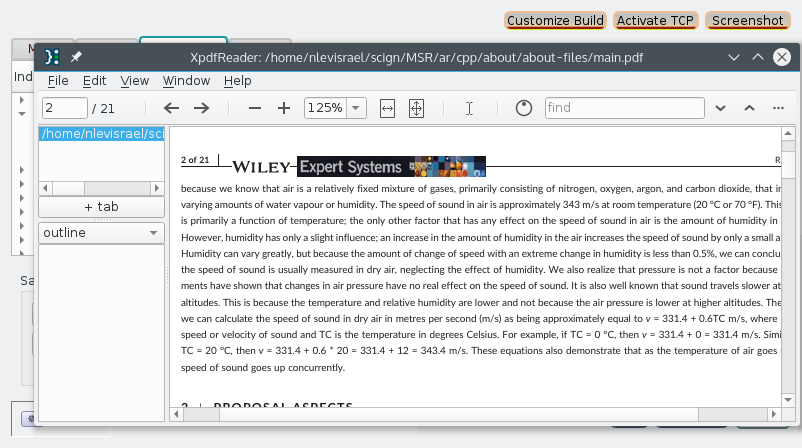
\includegraphics[scale=1.5]{texs/xpdf.png}}
            
  \node [text width=9.2cm,align=justify,fill=logoCyan!20, draw=logoBlue, 
  draw opacity=0.5,line width=1mm, fill opacity=0.9]
   at (0.3,0.82){\textbf{Each data set can be linked back to an original 
   article or other publication reporting on the data set and 
   experimental results.
   Different parts of the data set can be linked to 
   textual anchors in the publication.}};

  \node [text width=9.2cm,align=justify,fill=logoCyan!20, draw=logoBlue, 
  draw opacity=0.5,line width=1mm, fill opacity=0.9]
   at (0.7,0.42){In this example, 
   after viewing a short description of a particular data field 
   inside the Dataset Application, researchers have the option 
   of studying that parameter further by reading at the location 
   in the original publication where the field is introduced or described.  
   The XPDF viewer is compiled as an embedded application 
   within the main Dataset Application and can itself be customized 
   for each data set.};

            \annotatedFigureBox{0.2,0.12}{0.98,0.65}{1}{0.59,0.665}%            
      %      \annotatedFigureBox{0.222,0.284}{0.3743,0.4934}{B}{0.3743,0.4934}%tr
      %      \annotatedFigureBox{0.555,0.784}{0.6815,0.874}{C}{0.555,0.784}%bl
      %      \annotatedFigureBox{0.557,0.322}{0.8985,0.5269}{D}{0.8985,0.5269}%tr
  
        \end{annotatedFigure}

   %     \caption{Expanded Sample (A)}
    %    \label{fig:teaser}

    \end{frame}


